\documentclass[paper=a4, fontsize=10pt]{scrartcl} % A4 paper and 11pt font size

\usepackage[T1]{fontenc} % Use 8-bit encoding that has 256 glyphs
\usepackage{fourier} % Use the Adobe Utopia font for the document - comment this line to return to the LaTeX default
\usepackage[english]{babel} % English language/hyphenation
\usepackage{amsmath,amsfonts,amsthm} % Math packages
\usepackage{graphicx}
\usepackage[cm]{fullpage}
\usepackage{float}
\usepackage{sectsty} % Allows customizing section commands
\allsectionsfont{\centering \normalfont\scshape} % Make all sections centered, the default font and small caps

\usepackage{fancyhdr} % Custom headers and footers
\pagestyle{fancyplain} % Makes all pages in the document conform to the custom headers and footers
\fancyhead{} % No page header - if you want one, create it in the same way as the footers below
\fancyfoot[L]{} % Empty left footer
\fancyfoot[C]{} % Empty center footer
\fancyfoot[R]{\thepage} % Page numbering for right footer
\renewcommand{\headrulewidth}{0pt} % Remove header underlines
\renewcommand{\footrulewidth}{0pt} % Remove footer underlines
\setlength{\headheight}{13.6pt} % Customize the height of the header

\numberwithin{equation}{section} % Number equations within sections (i.e. 1.1, 1.2, 2.1, 2.2 instead of 1, 2, 3, 4)
\numberwithin{figure}{section} % Number figures within sections (i.e. 1.1, 1.2, 2.1, 2.2 instead of 1, 2, 3, 4)
\numberwithin{table}{section} % Number tables within sections (i.e. 1.1, 1.2, 2.1, 2.2 instead of 1, 2, 3, 4)

\setlength\parindent{0pt} % Removes all indentation from paragraphs - comment this line for an assignment with lots of text

%----------------------------------------------------------------------------------------
%	TITLE SECTION
%----------------------------------------------------------------------------------------

\newcommand{\horrule}[1]{\rule{\linewidth}{#1}} % Create horizontal rule command with 1 argument of height

\title{	
\normalfont \normalsize 
\textsc{Radboud University Nijmegen}  % Your university, school and/or department name(s)
\horrule{0.5pt} \\[0.3cm] % Thin top horizontal rule
\huge Statistical Machine Learning \\ Assignment 2 \\ % The assignment title
\horrule{2pt}  % Thick bottom horizontal rule
}

\author{Steven Reitsma \\ (s4132343)} % Your name

\date{\normalsize\today} % Today's date or a custom date

\begin{document}

\maketitle % Print the title

\section{Sequential learning}
\subsection{Obtaining the prior}
\begin{enumerate}
	\item 
		\begin{align}
			\boldsymbol{\tilde \Lambda} &= \boldsymbol{\tilde \Sigma}^{-1}\\
						   &= \begin{pmatrix}
								   60 &  50 & -48 &  38\\
								   50 &  50 & -50 &  40\\
								  -48 & -50 &  52.4 & -41.4\\
								   38 &  40 & -41.4 &  33.4\\
							  \end{pmatrix}
		\end{align}

		Using the precision matrix we can use equations 2.69, 2.73 and 2.75 from Bishop to compute the mean and covariance of the conditional distribution $p([x_1, x_2]^T \vert x_3 = x_4 = 0)$.

		\begin{align}
			\boldsymbol\Sigma_p &= \boldsymbol\Lambda_{aa}^{-1} \tag{according to 2.73}\\
			\boldsymbol\Lambda_{aa} &= \begin{pmatrix}
								60 & 50 \\
								50 & 50
							\end{pmatrix} \\
			\boldsymbol\Sigma_p &= \begin{pmatrix}
							0.1 & -0.1 \\
   							-0.1 &    0.12 \
   						\end{pmatrix}
		\end{align}

		\begin{align}
			\boldsymbol\mu_p = \boldsymbol\mu_{a} - \boldsymbol\Lambda_{aa}^{-1} \boldsymbol\Lambda_{ab} (\boldsymbol x_{b} - \boldsymbol\mu_{b}) \tag{according to 2.75}\\
		\end{align}
		In this equation, $a$ is the first partition and $b$ is the second partition when partitioned according to equation 2.65.
		\begin{align}
			\boldsymbol\mu_p &= \begin{pmatrix} 1 \\ 0 \end{pmatrix} - \begin{pmatrix} 60 & 50 \\ 50 & 50 \end{pmatrix}^{-1} \begin{pmatrix} -48 & 38 \\ -50 & 40 \end{pmatrix} (\begin{pmatrix} 0 \\ 0 \end{pmatrix} - \begin{pmatrix} 1 \\ 2 \end{pmatrix}) \\
			 &= \begin{pmatrix} 1 \\ 0 \end{pmatrix} - \begin{pmatrix} 0.1 & -0.1 \\ -0.1 & 0.12 \end{pmatrix} \begin{pmatrix} -48 & 38 \\ -50 & 40 \end{pmatrix} (\begin{pmatrix} 0 \\ 0 \end{pmatrix} - \begin{pmatrix} 1 \\ 2 \end{pmatrix}) \\
			 &= \begin{pmatrix} 0.8 \\ 0.8 \end{pmatrix}
		\end{align}
	\item Using the numpy-equivalent of \verb|mvnrnd| I obtained $\boldsymbol\mu_t$.

			\begin{verbatim}
				np.random.multivariate_normal(mu, sigma, 1)
			\end{verbatim}

			returned:

			\begin{equation}
				\boldsymbol\mu_t = \begin{pmatrix} 0.78848608 \\ 0.87686679 \end{pmatrix}
			\end{equation}
	\item The plot shows a thin `strip' as illustrated in figure \ref{gaussian}. The density is highest at the mean, and the density decreases quickly as both x and y increase, or as both x and y decrease. The density decreases less quickly as $x \text{ XOR } y$ decreases. This makes sense when we look at $\boldsymbol\Sigma_p$.
			\begin{figure}[h!]
				\centering
				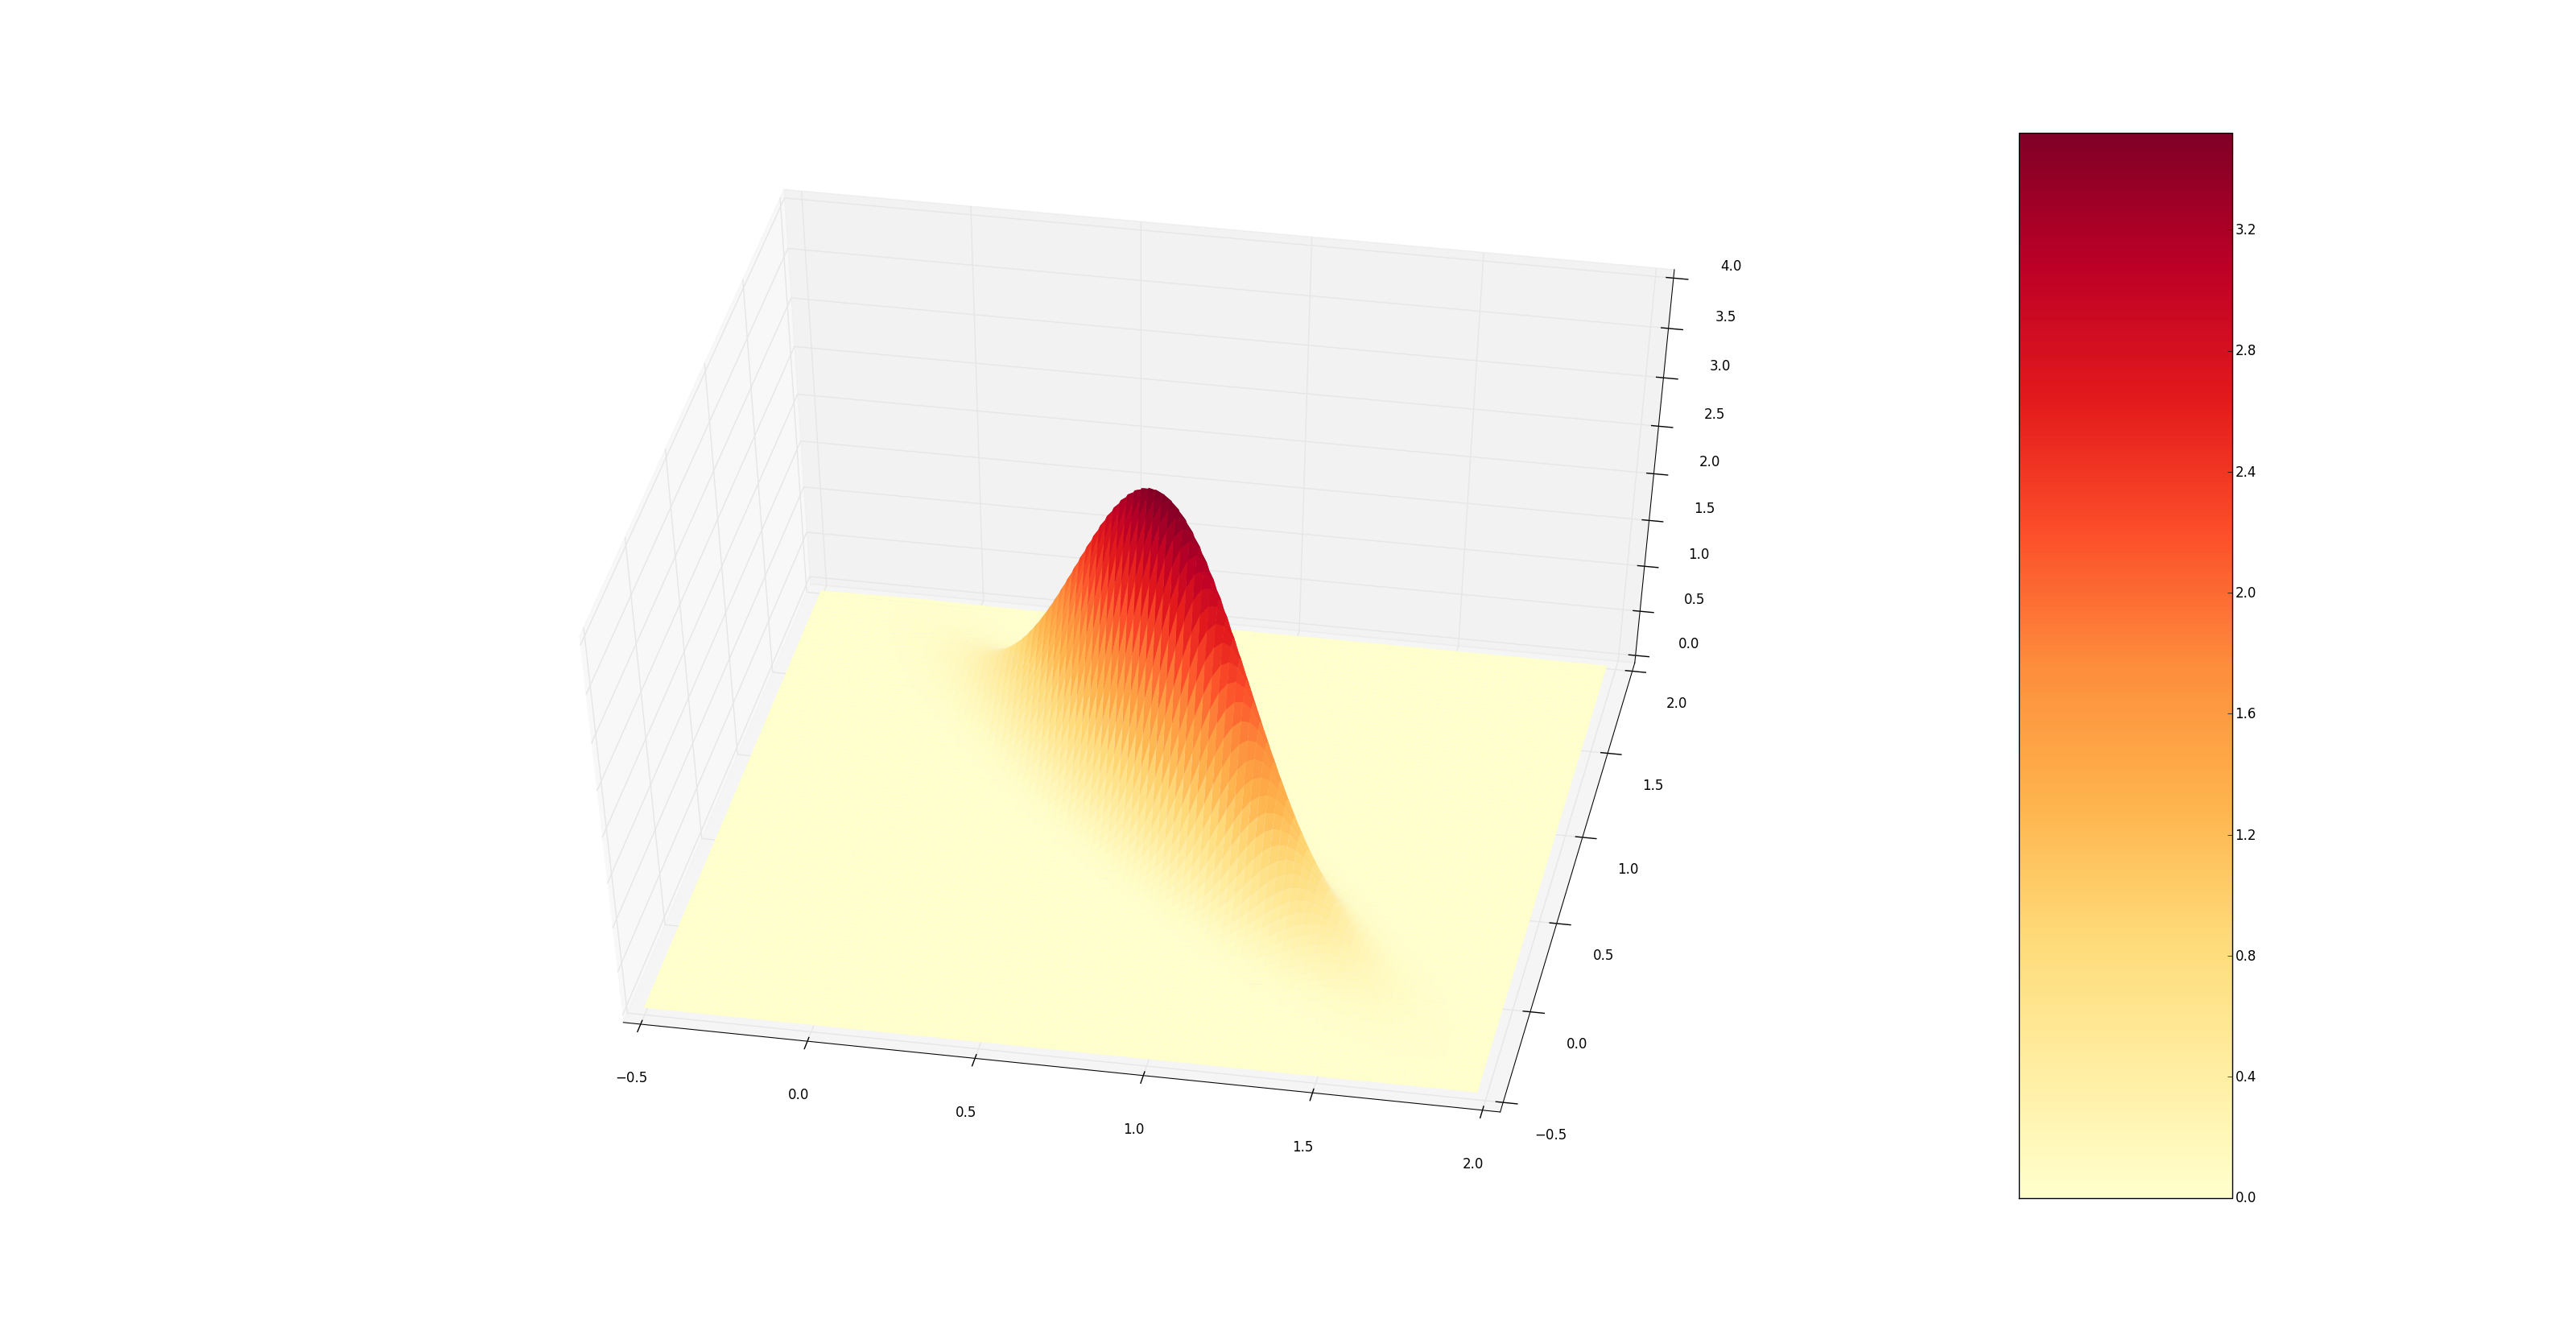
\includegraphics[width=\textwidth]{exercise_113_1.png}
				\label{gaussian}
				\caption{The probability density of the distribution. The axis on the bottom left is the x-axis.}
			\end{figure}
\end{enumerate}

\subsection{Generating the data}
\begin{enumerate}
	\item Small subset to illustrate the data:
			\begin{verbatim}
				-6.550125505999724318e-01,-3.266004957677250964e+00
				2.629696100570084738e+00,2.392902940429734171e-01
				1.336595266086160194e+00,4.689984757937132542e+00
				1.650219248260114124e+00,1.170028787392207059e+00
				1.299340276829215046e+00,-2.175267671986114149e-02
				1.729588572535984969e+00,4.837982469851976886e-01
				9.217728990799070043e-01,-5.346863389136486955e-01
				3.134103800140720097e-01,-1.955795492459505569e+00
				4.493626096671710535e+00,1.535380383556263162e+00
				-1.332499772337966126e+00,3.918138378413710043e+00
			\end{verbatim}
	\item This can easily be calculated using equations 2.121, 2.122 and 2.125.

			\begin{align}
				\boldsymbol\mu_{ML} &= \frac{1}{N} \sum_{n=1}^N \boldsymbol x_n \\
				&= (0.66690639, 0.90843429)^T
			\end{align}

			Calculated using the following Python script:
			\begin{verbatim}
				pairs = np.loadtxt('pairs.csv', delimiter=',')
				mu_ml = 1.0/np.size(pairs, 0) * sum(pairs)
				print mu_ml
			\end{verbatim}

			For the covariance matrix:

			\begin{align}
				\boldsymbol\Sigma_{ML} &= \frac{1}{N} \sum_{n=1}^N (\boldsymbol x_n - \boldsymbol \mu_{ML})(\boldsymbol x_n - \boldsymbol\mu_{ML})^T\\
				&= \begin{pmatrix} 2.06554144 & 0.84461216 \\ 0.84461216 & 3.930928 \end{pmatrix}
			\end{align}

			Calculated using the following Python script:
			\begin{verbatim}
				pairs = np.loadtxt('pairs.csv', delimiter=',')
				mu_ml = 1.0/np.size(pairs, 0) * sum(pairs)
				
				sigma_ml = 1.0/np.size(pairs, 0) * np.dot((pairs - mu_ml).T, (pairs - mu_ml))
				print sigma_ml
			\end{verbatim}

			For the unbiased covariance matrix:
			\begin{align}
				\boldsymbol \Sigma_U &= \frac{1}{N-1} \sum_{n=1}^N (\boldsymbol x_n - \boldsymbol \mu_{ML})(\boldsymbol x_n - \boldsymbol\mu_{ML})^T\\
				&= \begin{pmatrix} 2.06760905 & 0.84545762 \\ 0.84545762 & 3.93486286 \end{pmatrix}
			\end{align}

			Comparing with the true values for $\boldsymbol\mu_t$ and $\boldsymbol\Sigma_t$ we can see that the estimation for $\boldsymbol\Sigma_t$ is not that far off, as can be seen by the absolute error below:

			\begin{equation}
				\vert \boldsymbol\Sigma_t - \boldsymbol\Sigma_U \vert_{\text{elementwise}} =
				\begin{pmatrix}
					0.06554144 & 0.04461216 \\
					0.04461216 & 0.069072 
				\end{pmatrix}
			\end{equation}

			The error for the mean is slightly larger, especially for the first component:

			\begin{equation}
				\vert \boldsymbol\mu_t - \boldsymbol\mu_{ML} \vert_{\text{elementwise}} =
				\begin{pmatrix}
					0.12157969 \\
					0.03156750
				\end{pmatrix}
			\end{equation}
\end{enumerate}

\subsection{Sequential learning algorithms}

\begin{enumerate}
	\item Using equation 2.126 from Bishop I wrote the following piece of Python code:

			\begin{verbatim}
				def sequential_mean(pairs):
				    mu = 0
				    for i in range(1, np.size(pairs, 0)+1):
				        mu = mu + 1.0 / i * (pairs[i-1] - mu)
				        print mu
			\end{verbatim}

			This converges to the same result as the batch result. In a real world scenario the pairs would be read sequentially from the file as well.
	\item Matching the variables we get the following equations:

			\begin{align}
				p(\boldsymbol\mu) &= \mathcal{N} (\boldsymbol\mu \vert \boldsymbol\mu^{(n-1)}, \boldsymbol\Sigma^{(n-1)})\\
				p(\boldsymbol x_n \vert \boldsymbol\mu) &= \mathcal{N} (\boldsymbol x_n \vert \boldsymbol\mu, \boldsymbol\Sigma_t)\\
				p(\boldsymbol x_n) &= \mathcal{N} (\boldsymbol x_n \vert \boldsymbol\mu^{(n-1)}, \boldsymbol\Sigma_t + \boldsymbol\Sigma^{(n-1)})\\
				p(\boldsymbol\mu \vert \boldsymbol x_n) &= \mathcal{N} (\boldsymbol\mu \vert \boldsymbol S \{ \boldsymbol\Sigma_t^{-1} \boldsymbol x_n + \frac{1}{\boldsymbol\Sigma^{(n-1)}} \boldsymbol\mu^{(n-1)} \}, \boldsymbol S)\\
				\boldsymbol S &= (\frac{1}{\boldsymbol\Sigma^{(n-1)}} + \boldsymbol\Sigma_t^{-1})^{-1}
			\end{align}

			Using equation 1.21 we can compute $\boldsymbol \mu^{(n)}$.

			So our ``update-rules'' for the $\boldsymbol\mu$ and $\boldsymbol\Sigma$ are as follows:

			\begin{align}
				\boldsymbol\mu^{(n)} &= \boldsymbol S \{ \boldsymbol\Sigma_t^{-1} \boldsymbol x_n + \frac{1}{\boldsymbol\Sigma^{(n-1)}} \boldsymbol\mu^{(n-1)} \}\\
				\boldsymbol\Sigma^{(n)} &= \boldsymbol S
			\end{align}
	\item Implementing in Python was easy using the two equations above. As a result for the final $\boldsymbol\mu$ I got the following:

			\begin{align}
				\boldsymbol\mu = \begin{pmatrix} 0.67161114 \\ 0.91312478 \end{pmatrix}
			\end{align}

			The code snippet:

			\begin{verbatim}
					for i in range(1, np.size(pairs, 0)+1):
					    S = np.linalg.inv(np.linalg.inv(sigma[i-1]) + np.linalg.inv(sigma_t))
					    mu[i] = np.dot(S, (np.dot(np.linalg.inv(sigma_t), pairs[i-1]) +
					            np.dot(np.linalg.inv(sigma[i-1]), mu[i-1])))
					    sigma[i] = S

					    print mu[i]
			\end{verbatim}

			Note that \verb|np.dot| is equivalent to Matlab's *-operator.
	\item This would be more clear in two separate plots, but since the assignment requires a single graph I have done as requested.
		  In figure \ref{map} it is clear that the MAP estimation performs better when the number of data points is low. This makes sense since the MAP estimation is like a regularized version of the ML estimator. For a higher number of data points, the difference is very small.

			\begin{figure}[ht!]
				\centering
				\hspace*{-10em}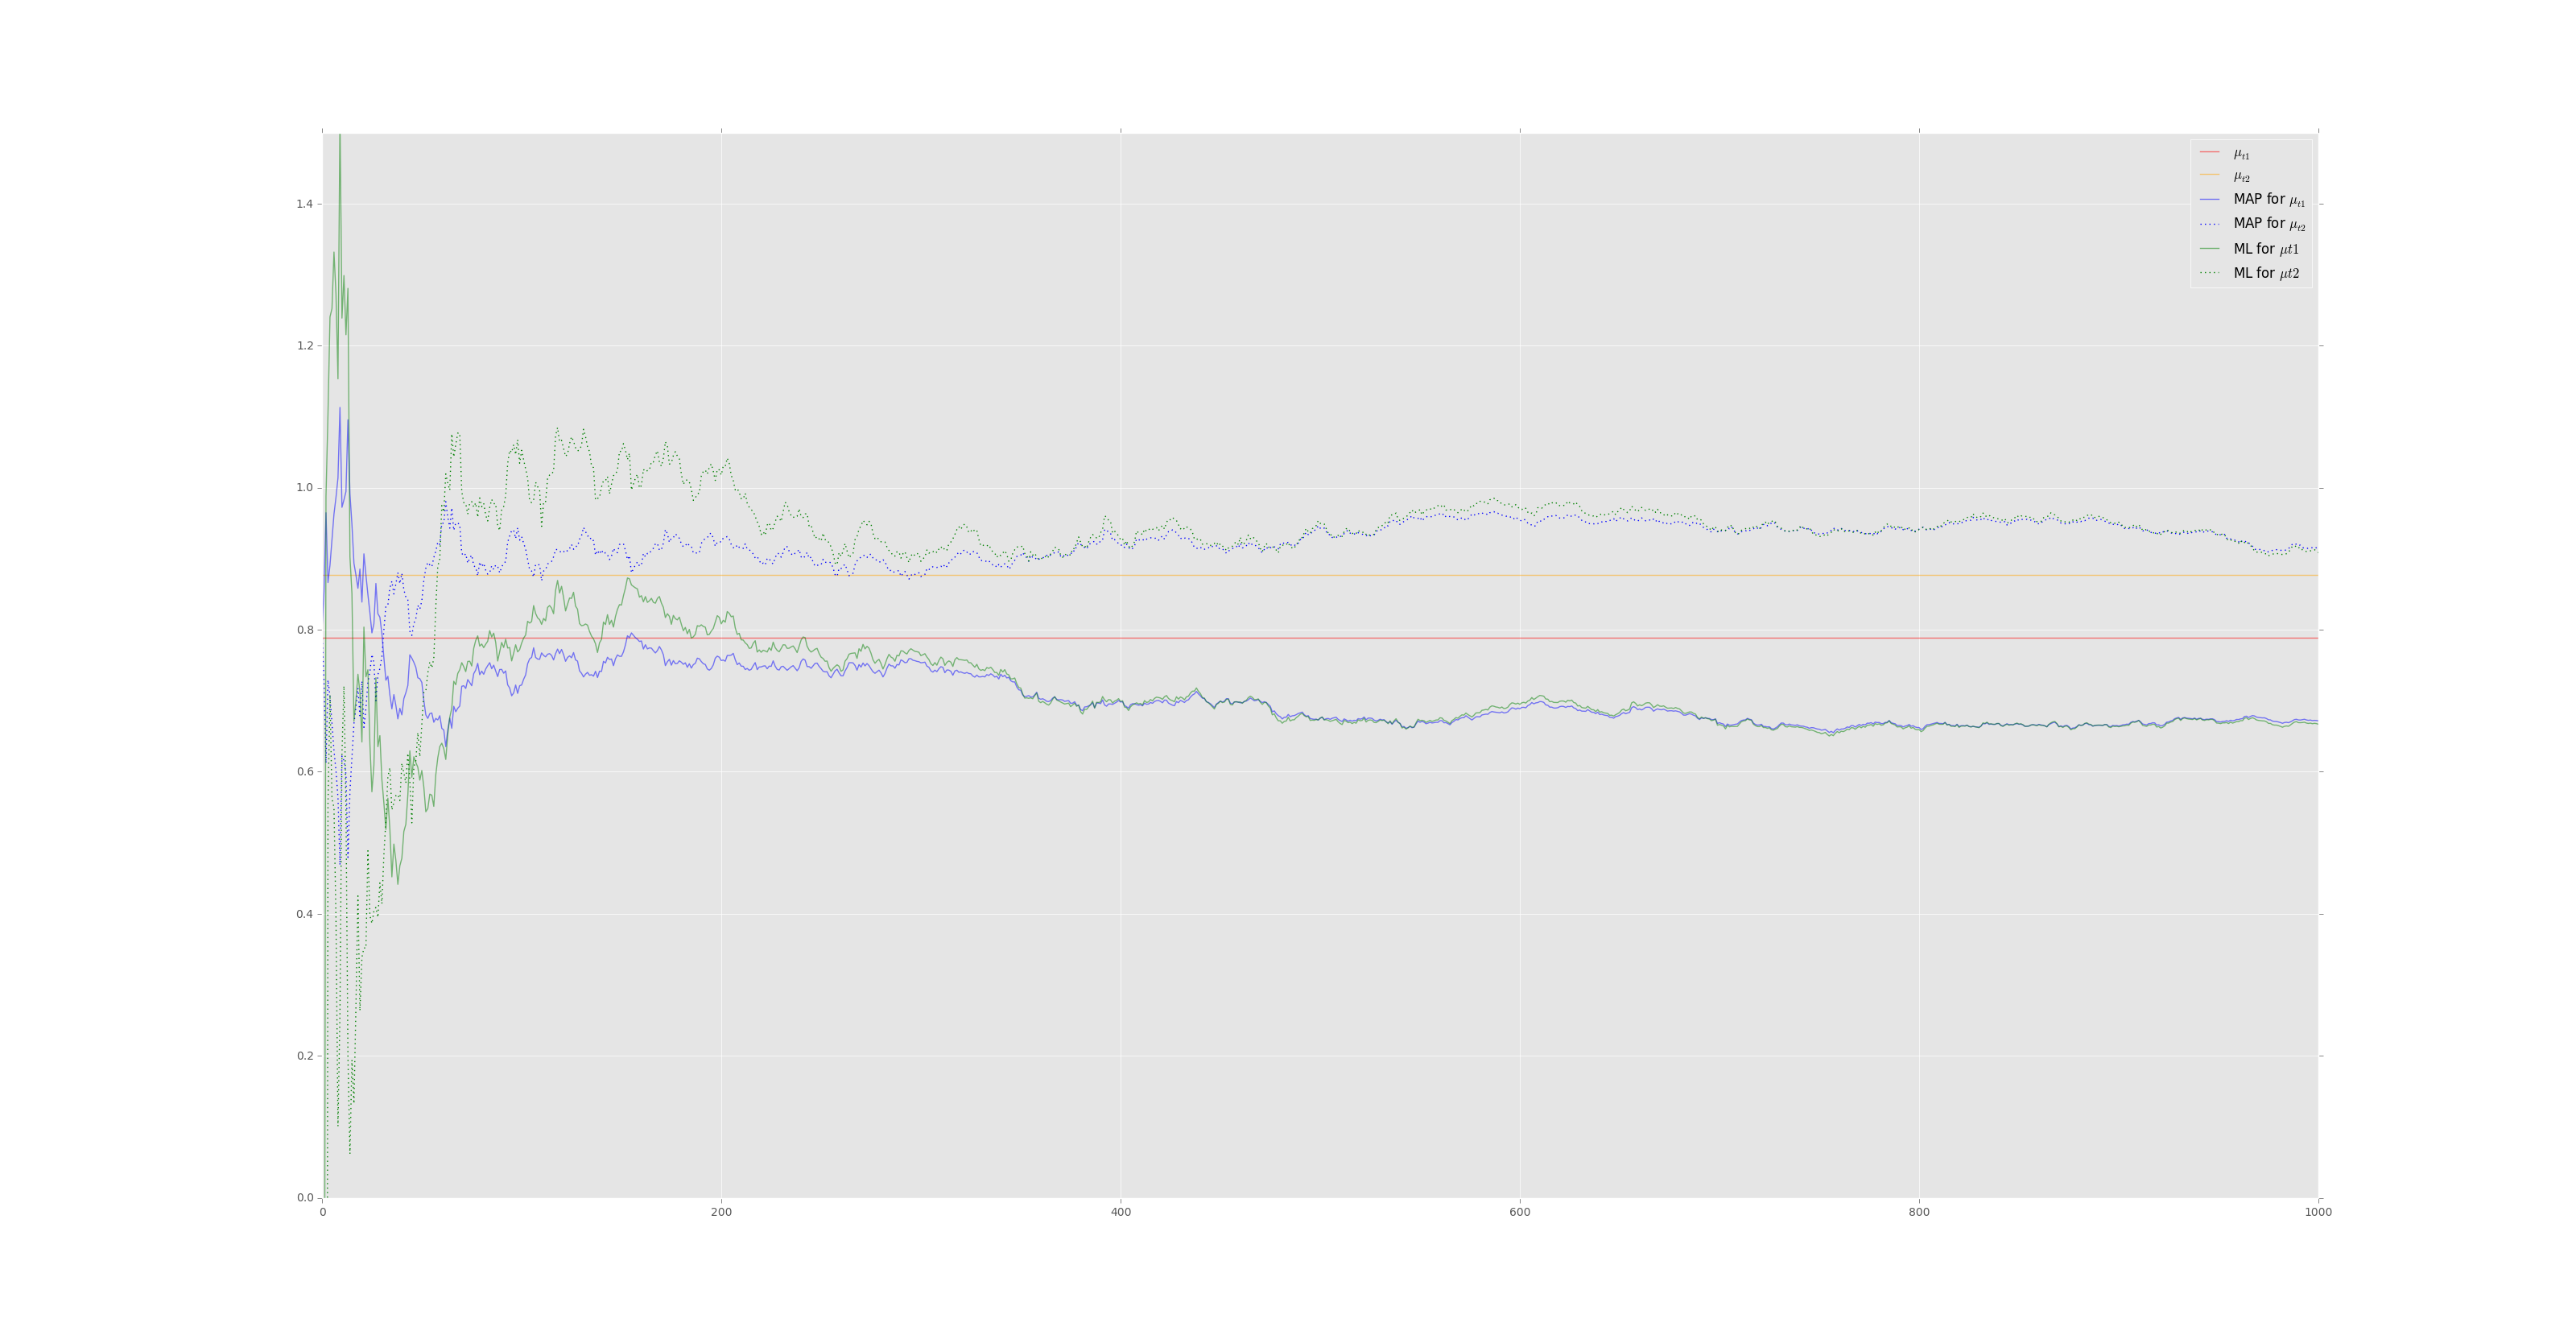
\includegraphics[width=1.3\textwidth]{exercise_134.png}
				\caption{The two dotted lines show the MAP (blue) and ML (green) estimations for $\mu_{t1}$ while the solid lines show the estimations for $\mu_{t2}$. You can zoom in on the .pdf to show the figure more clearly.}
				\label{map}
			\end{figure}
\end{enumerate}

\section{The faulty lighthouse}
\subsection{Constructing the model}
\begin{enumerate}
	\item It is a reasonable distribution since the following should (and does) hold:
			\begin{align}
				\int_{-\frac{1}{2}\pi}^{\frac{1}{2}\pi} \frac{1}{\pi} \, dx &= 1 \tag{To be proven}\\
				&= \left. \frac{x}{\pi} + C \right|_{-\frac{1}{2}\pi}^{\frac{1}{2}\pi}\\
				&= \frac{1}{2} - - \frac{1}{2} = 1
			\end{align}
	\item 
			\begin{align}
				p_x(x) &= p_\theta(\theta_k) \, \bigg\vert \frac{d\theta}{dy} \bigg\vert \\
				&= p_\theta(g(x)) \, \big\vert g'(x) \big\vert \\
				g(x) &= \tan^{-1} \bigg(\frac{x_k - \alpha}{\beta}\bigg) \\
				g'(x) &= \frac{1}{1 + \bigg(\frac{x_k - \alpha}{\beta}\bigg)^2} \cdot \frac{1}{\beta} \\
				&= \frac{\beta}{\big(x_k - \alpha\big)^2 + \beta^2} \\
				p_\theta(g(x)) &= \frac{1}{\pi} \\
				p_x(x) &= \frac{\beta}{\big(x_k - \alpha\big)^2 + \beta^2} \cdot \frac{1}{\pi} \\
				&= \frac{\beta}{\pi \big[\big(x_k - \alpha\big)^2 + \beta^2\big]} \\
			\end{align}
	\item
			\begin{align}
				p(a \vert \mathcal{D}, \beta) &= p(\mathcal{D} \vert \alpha, \beta)p(\alpha \vert \beta) \\
				p(x_k \vert \alpha, \beta) &= \frac{\beta}{\pi \big[\big(x_k - \alpha\big)^2 + \beta^2\big]} \\
				&= \frac{\beta}{\pi} \cdot \frac{1}{\big[\big(x_k - \alpha\big)^2 + \beta^2\big]} \\
				\ln(p(x_k \vert \alpha, \beta)) &= \ln(\frac{\beta}{\pi} \cdot \frac{1}{\big[\big(x_k - \alpha\big)^2 + \beta^2\big]}) \\
				&= \ln(\frac{\beta}{\pi}) + \ln(\frac{1}{\big[\big(x_k - \alpha\big)^2 + \beta^2\big]}) \\
				&= \ln(\frac{\beta}{\pi}) - \ln(\big[\big(x_k - \alpha\big)^2 + \beta^2\big]) \\
				p(\mathcal{D} \vert \alpha, \beta) &= \prod_{x_k \in \mathcal{D}} p(x_k \vert \alpha, \beta) \\
				\ln(p(\mathcal{D} \vert \alpha, \beta)) &= \vert \mathcal{D} \vert \cdot \ln(\frac{\beta}{\pi}) - \sum_{x_k \in \mathcal{D}} \ln\big(\big[\big(x_k - \alpha\big)^2 + \beta^2\big]\big) 
			\end{align}

			Maximizing this gives the following expression:
			\begin{align}
				\hat \alpha = \arg\max_\alpha \bigg[ \, \vert \mathcal{D} \vert \cdot \ln(\frac{\beta}{\pi}) - \sum_{x_k \in \mathcal{D}} \ln\big(\big[\big(x_k - \alpha\big)^2 + \beta^2\big]\big) \bigg]
			\end{align}
	\item
			Using a simple Python script I got the following values:
				\begin{align}
					\hat\alpha &= 1.17137\\
					\bar\alpha &= -0.183333
				\end{align}

			With the following plot:

			\begin{figure}[ht!]
				\centering
				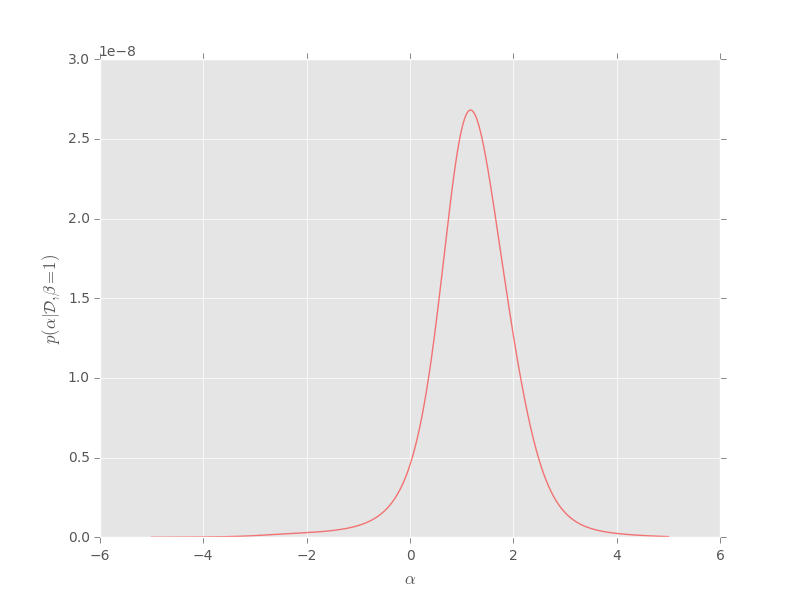
\includegraphics[scale=0.55]{exercise_214.png}
				\caption{$p(\alpha \vert \mathcal{D}, \beta = 1)$ plotted as a function of $\alpha$.}
			\end{figure}

			The mean and the maximum value differ because of the outliers in the data set. If we have a data set without many outliers (e.g. mean = median) then the mean of the data set and $\hat\alpha$ are approximately the same.
\end{enumerate}

\end{document}